\documentclass{article}
\usepackage[utf8]{inputenc}
\usepackage[russian]{babel}
\usepackage{amsfonts}
\usepackage{natbib}
\usepackage{upquote}
\usepackage{datetime}
\usepackage{multicol}
\usepackage{listings}
\usepackage{graphicx}

\setlength{\voffset}{-2cm}
\setlength{\textheight}{700pt}

\title{Численные методы: Лабораторная работа №3}
\author{Группа 4001BV: Карина Пилюшонока \and Александр Степанов \and Борис
Кувшинников} \date \today

\begin{document}
\maketitle
\newpage
\tableofcontents
\newpage
\section{Описание задачи}
В данной лабораторной работе необходимо реализовать методы решения
обыкновенных дифференциальных уравнений: метод Эйлера и метод Башфорта.
В качестве проверочного задания необходимо взять следующее уравнение: 
$0.25x - 0.05x^2 = 0$, с начальным условием $y = 1$. Также использовать разный
шаг для вычислений: $h_1 = 0.05, h_2=0.001$. После произведенных расчетов
отобразить график ошибок для каждого метода. Для сравнения, использовать
аналитическую функцию $g(t) = \frac{0.25 \cdot \exp^{0.25
\cdot t}}{0.25 + 0.05 \cdot \exp^{0.25 \cdot t}}$, на интервале $[0; 30]$.

\section{Ход работы}

  \begin{figure}[h!]
    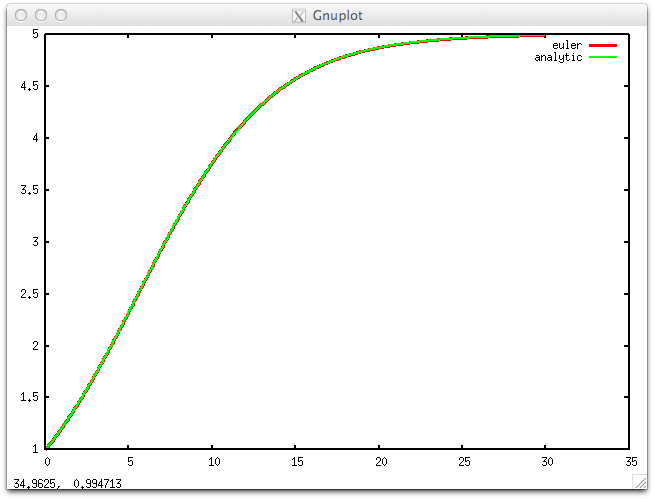
\includegraphics[width=13cm]{eulerVSanalytic005.png}
    \caption{Результат работы метода Эйлера и аналитическая функция с шагом
    $h=0.05$}
    \label{eulerVSanalytic}
  \end{figure}
  
  \begin{figure}
    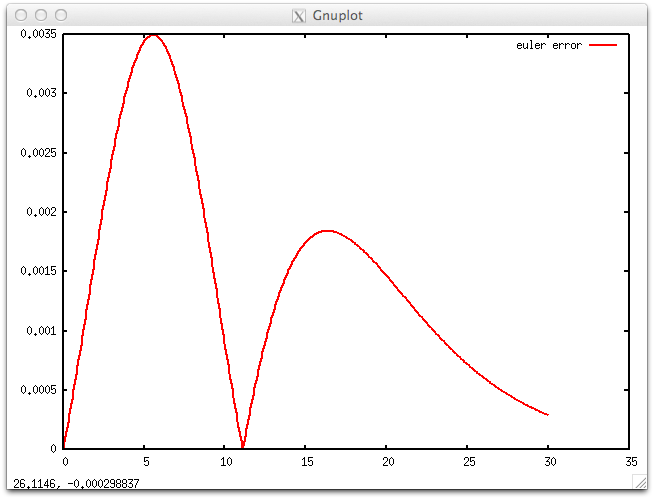
\includegraphics[width=13cm]{eulerError005.png}
    \caption{Ошибка работы метода Эйлера относительно аналитической функции с
    шагом $h=0.05$}
  \end{figure}
  
  \begin{figure}
    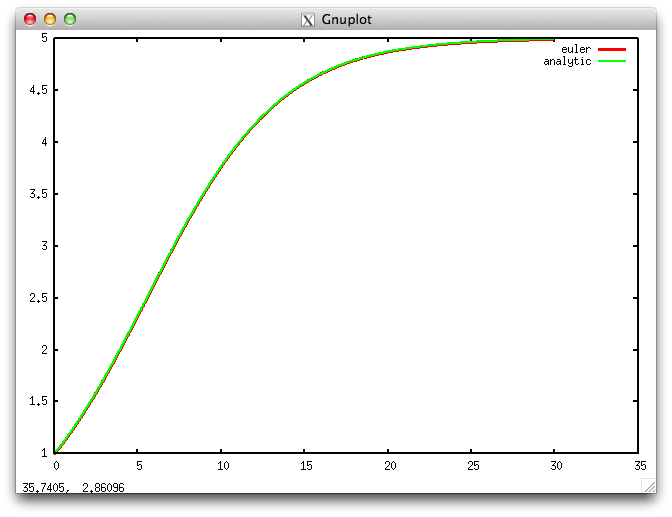
\includegraphics[width=13cm]{eulerVSanalytic0001.png}
    \caption{Результат работы метода Эйлера и аналитическая функция с шагом
    $h=0.001$}
    \label{eulerVSanalytic}
  \end{figure}
  
  \begin{figure}
    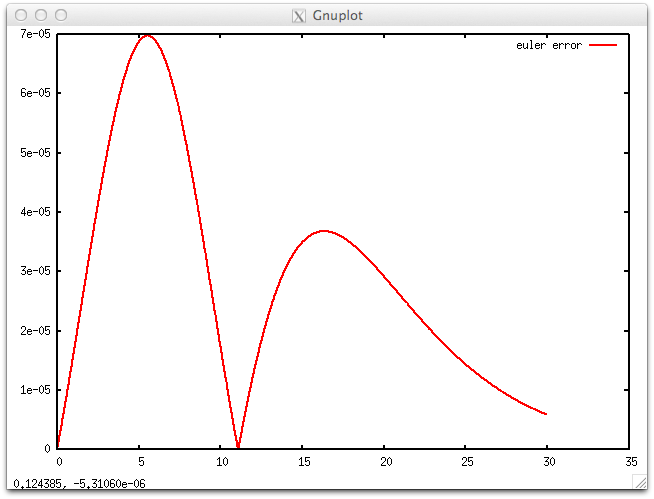
\includegraphics[width=13cm]{eulerError0001.png}
    \caption{Ошибка работы метода Эйлера относительно аналитической функции с
    шагом $h=0.001$}
  \end{figure}

  \begin{figure}
    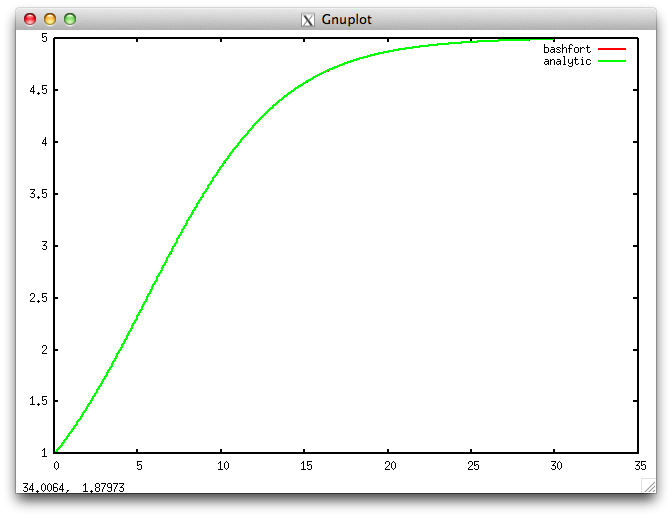
\includegraphics[width=13cm]{bashfortVSanalytic005.png}
    \caption{Результат работы метода Башфорта и аналитическая функция с шагом
    $h=0.05$}
    \label{eulerVSanalytic}
  \end{figure}
  
  \begin{figure}
    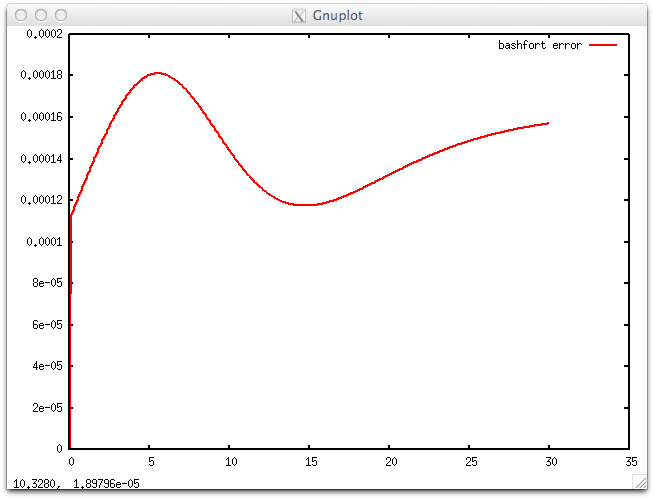
\includegraphics[width=13cm]{bashfortError005.png}
    \caption{Ошибка работы метода Башфорта относительно аналитической функции с
    шагом $h=0.05$}
  \end{figure}
  
  \begin{figure}
    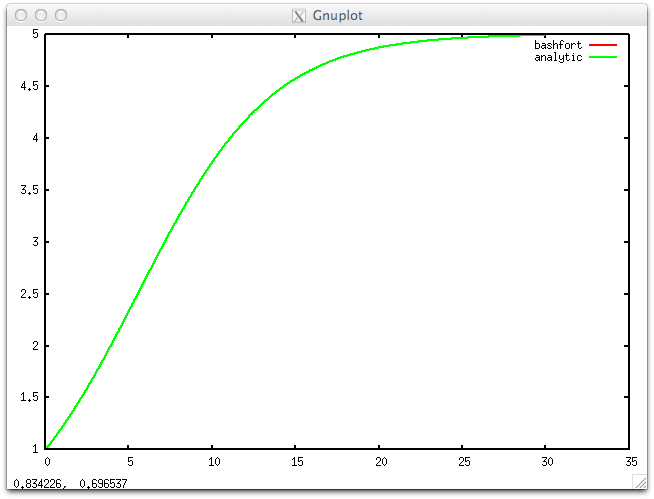
\includegraphics[width=13cm]{bashfortVSanalytic0001.png}
    \caption{Результат работы метода Башфорта и аналитическая функция с шагом
    $h=0.001$}
    \label{eulerVSanalytic}
  \end{figure}
  
  \begin{figure}
    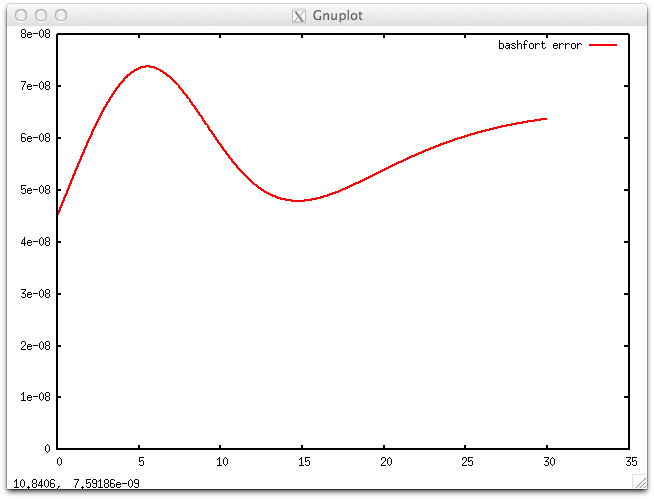
\includegraphics[width=13cm]{bashfortError0001.png}
    \caption{Ошибка работы метода Башфорта относительно аналитической функции с
    шагом $h=0.001$}
  \end{figure}

\newpage
\section{Вывод}
Проанализировав итоговый график ошибок, можно сказать, что метод Башфорта
генерирует наименьшую ошибку из анализируемых методов.
  \begin{figure}[h!]
    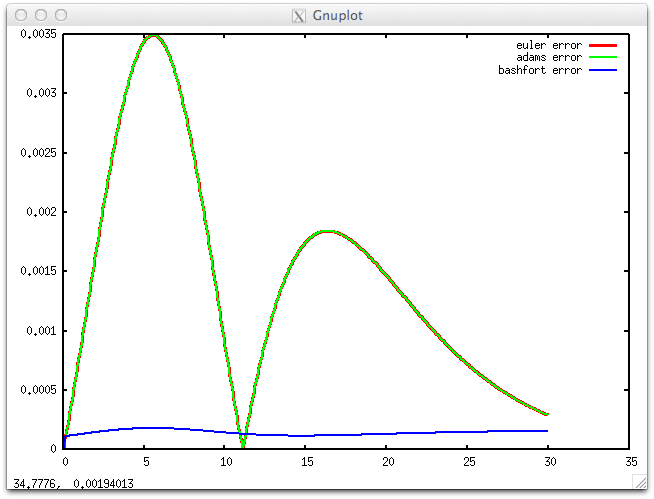
\includegraphics[width=12.8cm]{compareall.png}
    \caption{Сводный график ошибок методов при шаге $h=0.05$}
  \end{figure}
  
\newpage
\section{Исходный код}
\subsection{Метод Эйлера}
\begin{lstlisting}
function f(x) {
  return 0.25 * x - 0.05 * Math.pow(x,2)
}

var h = 0.1

var a = 0, b = 30

var y = [1]

function euler(h, a, b, f, y){
  for(var i=a; i<b; i+=h){
    var prevY = y[y.length-1]
    y.push(prevY + h * f(prevY))
  }
  return y
}

module.exports = euler
\end{lstlisting}

\subsection{Метод Адамса}
\begin{lstlisting}
var euler = require('./euler')
function f(x) {
  return 0.25 * x - 0.05 * Math.pow(x,2)
}

function df(x) {
  return 0.25 * Math.pow(x, 2) - 0.05 * Math.pow(x,3)
}

var h = 0.1

var a = 0, b = 30

var y = [1]

function adams(h, a, b, f, y){
  var eulerVal = euler(h,a,b,f,y)
  var k = 0
  y.push(eulerVal[++k])
  y.push(eulerVal[++k])
  y.push(eulerVal[++k])
  for(var i=a+(3*h); i<b; i+=h) {
    var prevY = y[k]
    var prevY1 = y[k-1]
    var prevY2 = y[k-2]
    var prevY3 = y[k-3]
    y.push(prevY + h/24*( 55*f(prevY) - 59*f(prevY1) + 37*f(prevY2) -9*(prevY3)))
    k++
  }
  return y
}

module.exports = adams

\end{lstlisting}

\subsection{Метод Башфорта}
\begin{lstlisting}
var adams = require('./adams')
var euler = require('./euler')

function f(x) {
  return 0.25 * x - 0.05 * Math.pow(x,2)
}

function df(t) {
  return (0.25 * y[0] *  Math.pow(Math.E, 0.25 * t ) /( 0.25 + 0.05 * y[0] * (Math.pow(Math.E,0.25*t) -1)))
}

var h = 0.1

var a = 0, b = 30

var y = [1]

function bashfort(h, a, b, f, y){
  var eu = [1]
  var eulerVal = euler(h,a,b,f,eu)
  
  var k = 0
  y.push(eulerVal[++k])
  y.push(eulerVal[++k])
  y.push(eulerVal[++k])
  for(var i=a+(3*h); i<b; i+=h){
    var prevY = y[k]
    var prevY1 = y[k-1] // y_{i-1}
    var prevY2 = y[k-2] // y_{i-2}
    var prevY3 = y[k-3]               
    var curY = prevY + h/24*( 55*f(prevY) - 59*f(prevY1) + 37*f(prevY2) -9*(prevY3)) // y_{i+1}
    curY = prevY + h/24*(9*f(curY) + 19*f(prevY) - 5*f(prevY1) + f(prevY2))
    curY = prevY + h/24*(9*f(curY) + 19*f(prevY) - 5*f(prevY1) + f(prevY2))
    y.push(curY) // y_{i+1} = ...
    k++
  }
}

bashfort(h, a, b, f, y)

var e = [1]
var eulerArr = euler(h, a, b, f, e)
var ad = [1]
var adamsArr = adams(h, a, b, f, ad)
console.log('x \t euler \t adams \t bashfort \t analytic')
for(var i=0, j=a; i < y.length; i++, j+=h) {
  console.log(''+ j + '\t' + eulerArr[i] + '\t' + adamsArr[i]+ '\t' + y[i] + '\t' + df(j))
}

module.exports = bashfort

\end{lstlisting}
\end{document}